\documentclass[aps,pra,reprint,groupedaddress,onecolumn,superscriptaddress]{revtex4-2}
\usepackage{graphicx}% Include figure files
\usepackage{dcolumn}% Align table columns on decimal point
\usepackage{bm}% bold math
\usepackage{amsmath}
\usepackage{siunitx}
\usepackage{enumitem}

\begin{document}

\title{Bullet-Point List of the Barium Network Paper}
\date{\today}

\maketitle

\section{Experimental Setup}

\subsection{Rb Laser (\SI{780}{\nano\meter} Reference)}
\begin{itemize}
    \item Stabilized via saturation absorption spectroscopy on the $5S_{1/2} \rightarrow 5P_{3/2}$ transition of $^{87}\text{Rb}$
    \item Reproducibility: \SI{\sim100}{\kilo\hertz}
\end{itemize}

\subsection{Ba$^+$ Laser (\SI{1762}{\nano\meter} Probe)}
\begin{itemize}
    \item Primary reference: single trapped $^{138}\text{Ba}^+$ ion, stabilized to the $6S_{1/2} \rightarrow 5D_{5/2}$ electric quadrupole transition
    \item Short-term stability provided by a ULE cavity; systematic uncertainties < \num{1e-15}
\end{itemize}

\subsection{Interferometer}
\begin{itemize}
    \item Dual-wavelength Michelson interferometer (modified NIST LM10 design)
    \item Optical path difference: \SI{4.2}{\meter} (representative of metropolitan-scale quantum links)
    \item Air-floated mirror stage (\SI{120}{\centi\meter} travel) minimizes vibrational noise
    \item Fringe detection: Si photodiode (\SI{780}{\nano\meter}), InGaAs photodiode (\SI{1762}{\nano\meter})
    \item Frequency counter: Hewlett Packard 53131A, two channels, 10 digits/s resolution, \SI{225}{\mega\hertz} bandwidth.
\end{itemize}

\subsection{Ambient Sensor}
\begin{itemize}
    \item BME280 sensor, co-located with interferometer beam path (within \SI{10}{\centi\meter})
    \item Temperature: uncertainty \SI{\pm 1}{\degreeCelsius}
    \item Humidity: uncertainty \SI{\pm 3}{\percent} RH
    \item Pressure: uncertainty \SI{\pm 0.6}{\hecto\pascal}
    \item Backup sensors: DHT22 (\SI{\pm 0.5}{\degreeCelsius}, \SI{\pm 1}{\percent} RH)
\end{itemize}

\subsection{Synchronization}
\begin{itemize}
    \item GPS-disciplined oscillator (\SI{10}{\mega\hertz} universal timebase) synchronizes all data acquisition
    \item Central time-series database (InfluxDB) for correlated analysis
\end{itemize}

\section{Data Collection}
\subsection{Dataset}
\begin{itemize}
    \item Training Dataset: \num{89106} synchronized measurements
    \item Validation Dataset: \num{46999} synchronized measurements (\SI{15}{days}, temporally separated)
\end{itemize}

\subsection{Environmental Ranges}
\begin{itemize}
    \item Temperature: \SIrange{15}{35}{\degreeCelsius}
    \item Relative humidity: \SIrange{20}{45}{\percent}
    \item Pressure: \SIrange{965}{1000}{\hecto\pascal}
\end{itemize}

\subsection{Sampling Rates}
\begin{itemize}
    \item Environmental parameters: \SI{1}{\hertz}
    \item Interferometric fringes: \SI{\sim 0.06}{\hertz} (every \SI{17}{\second}, limited by integration time)
\end{itemize}

\subsection{Data Preprocessing}
Timestamp alignment via linear interpolation, outlier removal using adaptive statistical thresholds

\section{Data Analysis}
\subsection{Refractive Index Calculation}
\begin{itemize}
    \item $n_{1762} = \frac{n_{780}}{\text{Ratio}} \frac{f_{780}}{f_{1762}}$, where Ratio = $N_{780}/N_{1762}$ (fringe counts from the frequency counter)
    \item $n_{780}$ computed from environmental parameters using Ciddor equation
\end{itemize}

\subsection{Regression Model}
\begin{itemize}
    \item Multivariate linear regression: $n = \alpha_0 + \alpha_T T + \alpha_H H + \alpha_P P$
    \item Goodness-of-fit: $R^2 = \num{0.996}$, F-statistic = \num{7.530e6} ($p < \num{0.001}$)
    \item Residual standard error: $\sigma_n \approx \num{1.2e-9}$
\end{itemize}

\subsection{Statistical Validation}
\begin{itemize}
    \item HAC (Heteroskedasticity and Autocorrelation Consistent) standard errors applied (lag = \numrange{18}{37})
    \item Block bootstrap validation (\num{2000} samples, block length = \num{58}) confirmed robustness
    \item Residual diagnostics: Durbin-Watson = \num{1.130}, Breusch-Godfrey LM = \num{29734.5} ($p < \num{0.001}$)
\end{itemize}

\section{Results}
\subsection{Refractive Index Model at \SI{1762}{\nano\meter}}
\subsubsection{Coefficients (with \SI{95}{\percent} HAC CI)}
\begin{itemize}
    \item Temperature ($\alpha_T$): \SI{-8.940e-7}{\per\degreeCelsius} [\num{-8.942e-7}, \num{-8.938e-7}]
    \item Humidity ($\alpha_H$): \SI{-1.780e-8}{\per\percent} [\num{-1.796e-8}, \num{-1.764e-8}]
    \item Pressure ($\alpha_P$): \SI{+2.569e-7}{\per\hecto\pascal} [\num{2.557e-7}, \num{2.581e-7}]
\end{itemize}

\subsubsection{Uncertainty Budget}
\begin{itemize}
    \item Systematic uncertainty (dominant): \num{2.12e-7} (from spatial/temporal sensor mismatches)
    \item Coefficient precision: $\delta\alpha_T = \num{1.77e-10}$, $\delta\alpha_H = \num{1.81e-10}$, $\delta\alpha_P = \num{1.10e-10}$
\end{itemize}

\subsection{Humidity Weighting Difference}
\subsubsection{Experimental vs. Models}
\begin{itemize}
    \item Measured $\partial n/\partial H = \SI{-1.780e-8}{\per\percent}$
    \item Ciddor: \SI{-1.537e-8}{\per\percent} (\SI{+15.8}{\percent} discrepancy)
    \item Edlén: \SI{-1.526e-8}{\per\percent} (\SI{+16.6}{\percent} discrepancy)
    \item Mathar: \SI{-1.653e-8}{\per\percent} (\SI{+7.7}{\percent} discrepancy)
\end{itemize}

\subsubsection{Physical Origin}
\begin{itemize}
    \item Proximity to H$_2$O absorption lines at \SI{1761.0405}{\nano\meter} and \SI{1762.4852}{\nano\meter}
    \item Kramers-Kronig dispersion calculation: predicts \SI{+15.3}{\percent} enhancement over Ciddor
    \item Theoretical $\alpha_H^{\text{theory}} = \SI{-1.772e-8}{\per\percent}$ (within \SI{0.5}{\percent} of experiment)
\end{itemize}

\subsection{Post-Selection Phase Noise Compensation}
\subsubsection{Performance Metrics}
\paragraph{Long-term (\SI{15}{days})}
\begin{itemize}
    \item Phase noise reduction: \SI{80.97}{\percent}
    \item Phase standard deviation: \SI{17.938}{\radian} → \SI{3.414}{\radian} (\num{5.3}× improvement)
    \item Autocorrelation time: \SI{5668}{\second} → \SI{302}{\second}
    \item QEC threshold compliance: \SI{1.2}{\percent} → \SI{9.7}{\percent} of operational time
\end{itemize}

\paragraph{Short-term (\SI{12}{\hour})}
\begin{itemize}
    \item Phase noise reduction: \SI{60.20}{\percent}
    \item Phase standard deviation: \SI{6.548}{\radian} → \SI{2.606}{\radian} (\num{2.5}× improvement)
    \item Autocorrelation time: \SI{560}{\second} → \SI{1}{\second} (\num{560}× reduction, effective whitening)
    \item QEC threshold compliance: \SI{3.3}{\percent} → \SI{13.3}{\percent} of operational time
\end{itemize}

\subsubsection{Method}
Offline feed-forward subtraction using experimentally determined coefficients.

\newpage
\section{Figures}

\begin{figure}[ht]
\centering
\includegraphics[width=0.8\textwidth]{figures/fig1_nc.eps}
\caption{
Quantum-traceable metrology architecture for precision refractometry at the \SI{1762}{\nano\meter} barium-ion transition wavelength. 
\textbf{(Blue)} Laboratory-based quantum references: a GPS-disciplined oscillator provides a universal timebase, a single trapped Ba$^+$ ion stabilizes the \SI{1762}{\nano\meter} probe laser, and a Rb reference stabilizes the \SI{780}{\nano\meter} reference laser. 
\textbf{(Red)} Field-deployable sensor node: a dual-wavelength interferometer with co-located environmental sensors ($T$, $H$, $P$) measures refractive index changes under realistic outdoor conditions. 
\textbf{(Yellow)} Central analysis unit: processes the validation dataset to establish precise environmental-phase relationships. 
This integrated system bridges quantum-grade stability and field deployment, enabling the part-per-billion precision ($\delta n \sim 1 \times 10^{-9}$) demonstrated in this work.
}
\label{fig:exp_setup}
\end{figure}

\begin{figure}[ht]
\centering
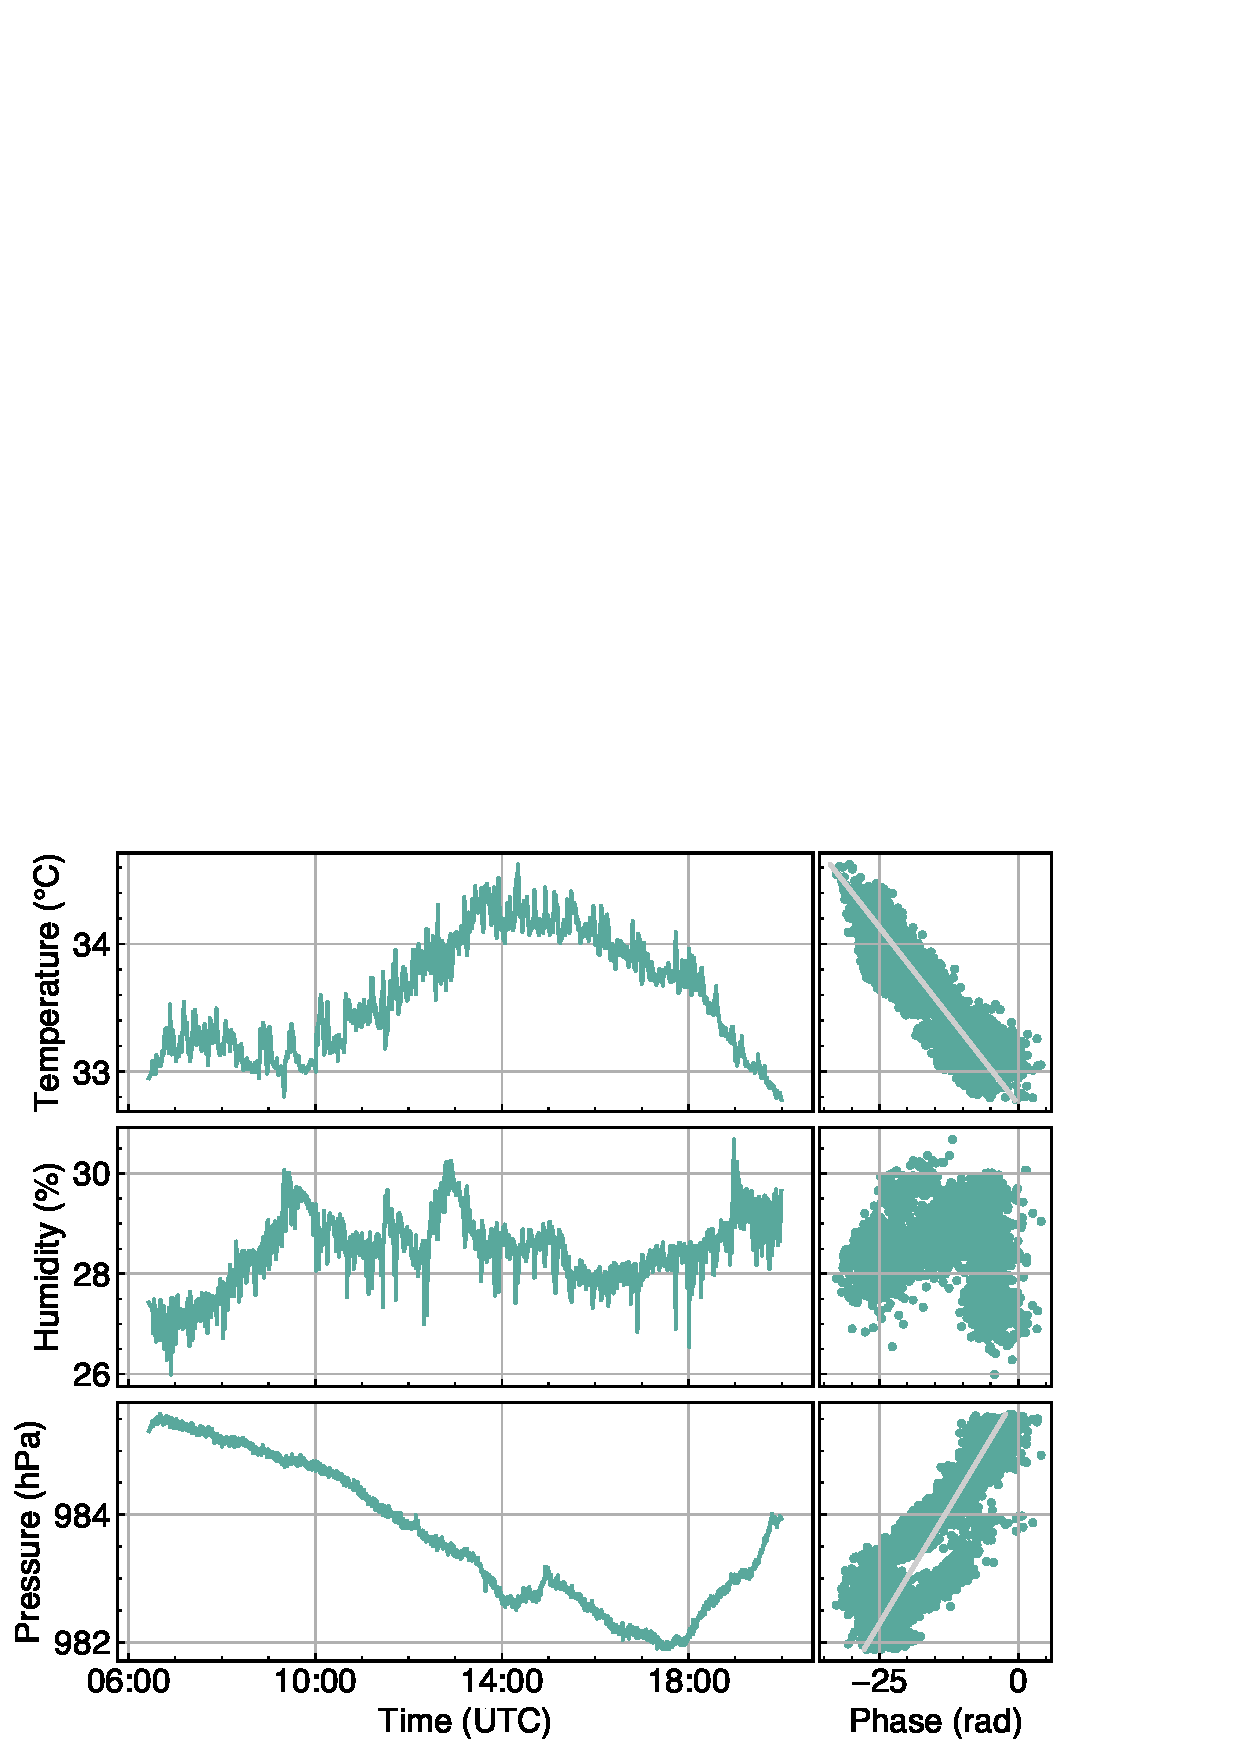
\includegraphics[width=0.8\textwidth]{figures/fig2_new.pdf}
\caption{
Environmental dynamics and their distinct correlations with measured refractive index at \SI{1762}{\nano\meter}.
\textbf{(a--c)} Synchronous \SI{14}{\hour} time-series measurements from the training dataset of atmospheric temperature (\SIrange{33}{34.5}{\celsius}), relative humidity (\SIrange{26}{31}{\percent}), and pressure (\SIrange{982}{986}{\hecto\pascal}) from the training dataset.
\textbf{(d)} Corresponding refractive index variations measured at \SI{1762}{\nano\meter}, expressed as $(n-1.0002)\times 10^{5}$, showing coherent temporal dynamics with environmental parameters.
\textbf{(e--g)} Quantitative correlation analysis between each environmental parameter and the resulting refractive index change. Phase noise exhibits a strong linear dependence on temperature ($R^{2} = 0.828$) and pressure ($R^{2} = 0.751$). The humidity-phase relationship, however, displays a characteristic non-linear pattern, deviating significantly from simple linear modeling.
\textbf{(h)} Self-correlation analysis of refractive index measurements, confirming measurement consistency ($R^{2} = 1.000$) and providing a validation baseline for environmental correlation studies.}
\label{fig:environmental_dynamics}
\end{figure}

\begin{figure}[ht]
\centering
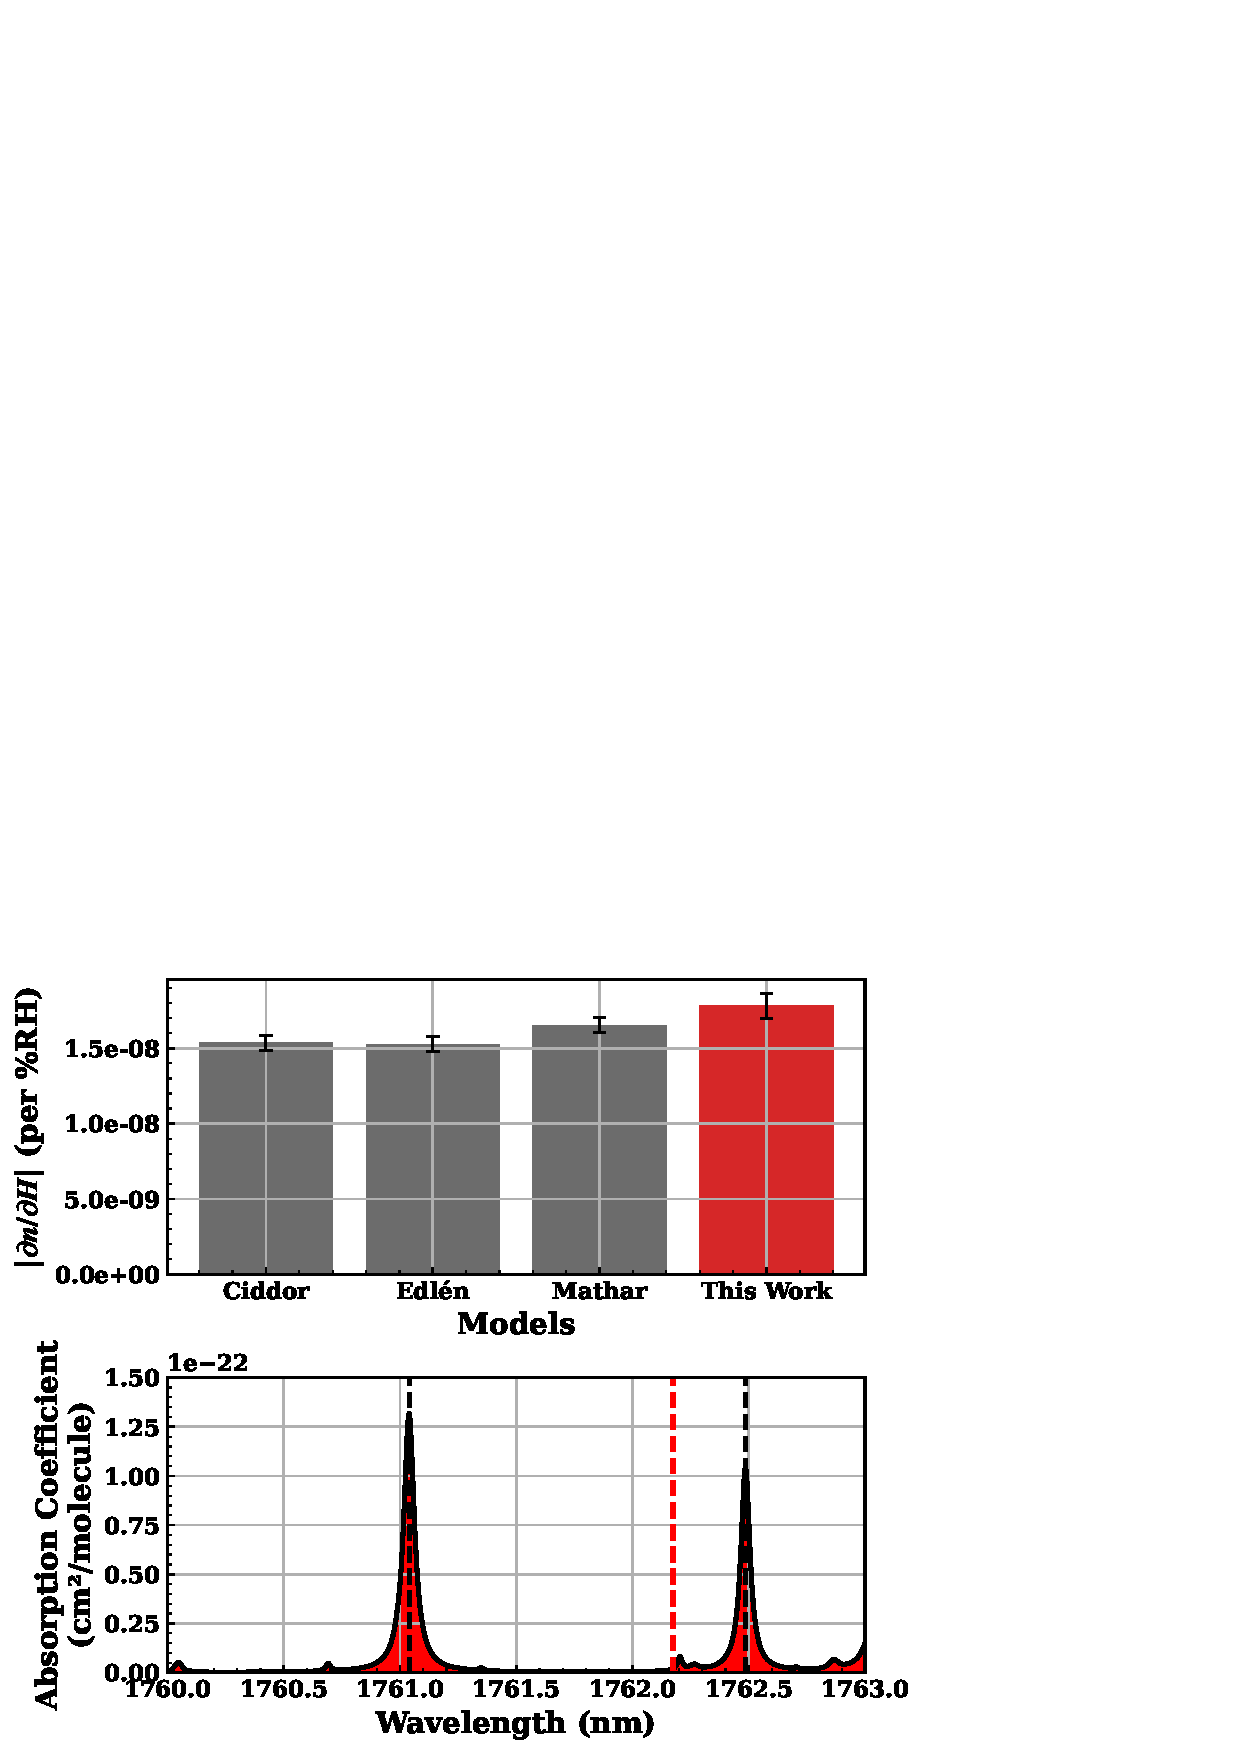
\includegraphics[width=0.8\textwidth]{figures/fig3_humidity_discrepancy.pdf}
\caption{
Systematic discrepancy in humidity sensitivity and its physical origin at \SI{1762}{\nano\meter}.
\textbf{(a)} Comparison of the experimentally derived humidity sensitivity coefficient with predictions from established empirical models. A significant enhancement is identified, while excellent agreement ($<\SI{1}{\percent}$ deviation) is found for temperature and pressure coefficients.
\textbf{(b)} Spectral analysis showing water vapor absorption features in the vicinity of the quantum-critical wavelength. The \SI{1762}{\nano\meter} transition lies between two strong absorption peaks at \SI{1761.0405}{\nano\meter} and \SI{1762.4852}{\nano\meter}, creating ideal conditions for Kramers-Kronig enhanced dispersion. Our first-principles calculation, performed over the full spectral range from \SI{1}{\micro\meter} to \SI{50}{\micro\meter}, explains the observed \SI{15.3}{\percent} increase in humidity sensitivity compared to the Ciddor model, or other standard atmospheric models.
}
\label{fig:humidity_discrepancy}
\end{figure}

\begin{figure}[ht]
\centering
\includegraphics[width=1\textwidth]{figures/combined_figure.png}
\caption{
Multi-scale phase noise characterization and suppression efficacy for quantum applications. 
\textbf{(a)} Long-term (\SI{15}{\day}) phase stability using the full validation dataset: time-domain performance showing environmental noise mitigation, with gray shaded region indicating the fault-tolerant threshold. 
\textbf{(b)} Long-term autocorrelation analysis: correlation time reduced from \SI{5668}{\second} to \SI{302}{\second}. 
\textbf{(c)} Long-term spectral characterization: power spectral density demonstrating substantial low-frequency noise suppression. 
\textbf{(d)} Short-term (\SI{12}{\hour}) phase dynamics from the validation dataset: optimized performance for quantum gate operations, with gray shaded region indicating the fault-tolerant threshold. 
\textbf{(e)} Short-term autocorrelation: dramatic noise whitening with correlation time reduced from \SI{560}{\second} to \SI{1}{\second}. 
\textbf{(f)} Short-term spectral analysis: frequency-domain transformation revealing noise structure modification. 
Key performance metrics: Long-term noise reduction of \SI{80.97}{\percent} ($\sigma_\phi$: \SI{17.938}{\radian} $\rightarrow$ \SI{3.414}{\radian}, 5.3$\times$) optimized for quantum memory applications. Short-term suppression achieves \SI{60.20}{\percent} reduction ($\sigma_\phi$: \SI{6.548}{\radian} $\rightarrow$ \SI{2.606}{\radian}, 2.5$\times$) ideal for quantum gate operations. QEC threshold compliance improved from \SI{1.2}{\percent} to \SI{9.7}{\percent} (long-term) and \SI{3.3}{\percent} to \SI{13.3}{\percent} (short-term). 
}
\label{fig:timeseries_comparison}
\end{figure}


\end{document}